\documentclass[twocolumn]{aastex61}
%\documentclass{emulateapj}
%\usepackage[colorlinks,urlcolor=blue,citecolor=blue,linkcolor=blue]{hyperref} 
\usepackage{graphicx,natbib}
\citestyle{aa}
\usepackage[space]{grffile}
\usepackage{latexsym}
\usepackage{amsfonts,amsmath,amssymb}
\usepackage{url}
\usepackage[utf8]{inputenc}
\usepackage{fancyref}
\usepackage{hyperref}
\usepackage{multirow}
\hypersetup{colorlinks=false,pdfborder={0 0 0},}

\newcommand{\rf}{\emph{realfast}}
\newcommand{\frb}{FRB 121102}

\begin{document}

\title{The \frb\ Observing Campaign: Multi-Telescope Radio Burst and Implications for the FRB Population}
%\title{Multi-Telescope Burst Properties and Implications for FRB Population}
\shorttitle{\frb\ Observing Campaign}
\shortauthors{Law et al.}

\author[0000-0002-4119-9963]{C.~J.~Law}
\affiliation{Dept of Astronomy and Radio Astronomy Lab, University of California, Berkeley, CA 94720, USA}

%\author{M.~W.~Abruzzo}
%\affiliation{Haverford College, 370 Lancaster Ave, Haverford, PA 19041, USA}

%\author{C.~G.~Bassa}
%\affiliation{ASTRON, Netherlands Institute for Radio Astronomy, Postbus 2, 7990 AA, Dwingeloo, The Netherlands}

%\author{S.~Bogdanov}
%\affiliation{Columbia Astrophysics Laboratory, Columbia University,  New York, NY 10027, USA}

\author{G.~C.~Bower}
\affiliation{Academia Sinica Institute of Astronomy and Astrophysics, 645 N. A'ohoku Place, Hilo, HI 96720, USA}

\author{S.~Burke-Spolaor}
\affiliation{National Radio Astronomy Observatory, Socorro, NM 87801, USA}
\affiliation{Department of Physics and Astronomy, West Virginia University, Morgantown, WV 26506, USA}
\affiliation{Center for Gravitational Waves and Cosmology, West Virginia University, Chestnut Ridge Research Building, Morgantown, WV 26505}

\author{B.~J.~Butler}
\affiliation{National Radio Astronomy Observatory, Socorro, NM 87801, USA}
\author{S.~Chatterjee}
\affiliation{Cornell Center for Astrophysics and Planetary Science and Department of Astronomy, Cornell University, Ithaca, NY 14853, USA}

\author{J.~M.~Cordes}
\affiliation{Cornell Center for Astrophysics and Planetary Science and Department of Astronomy, Cornell University, Ithaca, NY 14853, USA}

\author{P.~Demorest}
\affiliation{National Radio Astronomy Observatory, Socorro, NM 87801, USA}

\author{J.~W.~T.~Hessels}
\affiliation{ASTRON, Netherlands Institute for Radio Astronomy, Postbus 2, 7990 AA, Dwingeloo, The Netherlands}
\affiliation{Anton Pannekoek Institute for Astronomy, University of Amsterdam, Science Park 904, 1098 XH Amsterdam, The Netherlands}

\author{R.~Fender}
\affiliation{University of Oxford, UK}

%\author{V.~M.~Kaspi}
%\affiliation{Department of Physics and McGill Space Institute, McGill University, 3600 University St., Montreal, QC H3A 2T8, Canada}

%\author{A.~Keimpema}
%\affiliation{Joint Institute for VLBI ERIC, Postbus 2, 7990 AA Dwingeloo, The Netherlands}

%\author{H.~J.~van~Langevelde}
%\affiliation{Joint Institute for VLBI ERIC, Postbus 2, 7990 AA Dwingeloo, The Netherlands}
%\affiliation{Sterrewacht Leiden, Leiden University, Postbus 9513, 2300 RA, Leiden, the Netherlands}

\author{T.~J.~W.~Lazio}
\affiliation{Jet Propulsion Laboratory, California Institute of Technology, Pasadena, CA 91109, USA}

%\author[0000-0001-9814-2354]{B.~Marcote}
%\affiliation{Joint Institute for VLBI ERIC, Postbus 2, 7990 AA Dwingeloo, The Netherlands}

\author{D.~Michilli}
\affiliation{ASTRON, Netherlands Institute for Radio Astronomy, Postbus 2, 7990 AA, Dwingeloo, The Netherlands}
\affiliation{Anton Pannekoek Institute for Astronomy, University of Amsterdam, Science Park 904, 1098 XH Amsterdam, The Netherlands}

\author{M.~A.~McLaughlin}
\affiliation{Department of Physics and Astronomy, West Virginia University, Morgantown, WV 26506, USA}
\affiliation{Center for Gravitational Waves and Cosmology, West Virginia University, Chestnut Ridge Research Building, Morgantown, WV 26505}

\author{K.~Mooley}
\affiliation{University of Oxford, UK}

%\author{Z.~Paragi}
%\affiliation{Joint Institute for VLBI ERIC, Postbus 2, 7990 AA Dwingeloo, The Netherlands}

%\author{S.~M.~Ransom}
%\affiliation{National Radio Astronomy Observatory, Charlottesville, VA 22903, USA}

\author{M.~Rupen}
\affiliation{National Research Council of Canada, Herzberg Astronomy and Astrophysics, Dominion Radio Astrophysical Observatory, P.O. Box 248, Penticton, BC V2A 6J9, Canada}

\author{L.~G.~Spitler}
\affiliation{Max-Planck-Institut f\"ur Radioastronomie, Auf dem H\"ugel 69, D-53121 Bonn, Germany}

\author{P.~Scholz}
\affiliation{National Research Council of Canada, Herzberg Astronomy and Astrophysics, Dominion Radio Astrophysical Observatory, P.O. Box 248, Penticton, BC V2A 6J9, Canada}

\author{A.~Seymour}
\affiliation{Arecibo Observatory, HC3 Box 53995, Arecibo, PR 00612, USA}
\affiliation{Max-Planck-Institut f\"ur Radioastronomie, Auf dem H\"ugel 69, Bonn, D-53121, Germany}

%\author{S.~P.~Tendulkar}
%\affiliation{Department of Physics and McGill Space Institute, McGill University, 3600 University St., Montreal, QC H3A 2T8, Canada}

\author{R.~S.~Wharton}
\affiliation{Cornell Center for Astrophysics and Planetary Science and Department of Astronomy, Cornell University, Ithaca, NY 14853, USA}


\begin{abstract}
The millisecond radio transients known as Fast Radio Bursts have recently emerged as a mysterious, new class of astrophysical transient. The discovery of repeating bursts from \frb\ has shown that at least some FRBs are not cataclysmic and opened potential for studying FRB properties via a homogenous sample of bursts. The recent localization of \frb\ with the Very Large Array has helped measure its distance and a host of intrinsic properties. This localization was made with 9 bursts seen by the VLA in coordination the Arecibo, Effelsberg, and AMI-LA observatories. We present a detailed analysis of these bursts, including the first simultaneous detection of an FRB with multiple telescopes. We show that the burst spectra typically have a broad Gaussian shape on the scale of $\sim500$~MHz with fine spectral structure consistent with either scintillation or unresolved temporal structure. We present the luminosity distribution and temporal statistics for \frb\ and argue that the whole FRB population is adequately described by a single class similar to \frb. We close with thoughts on optimal strategies to make new interferometric localizations of FRBs.
\end{abstract}

\section{Introduction}
Fast Radio Bursts (FRBs) are a new class of millisecond-duration radio transient with a dispersion measure (DM) that implies that they originate outside of our Galaxy. At extragalactic (and potentially cosmological) distances, they are not only unusually luminous, but they provide a new tracer of other galaxies and the intergalactic medium (IGM). In this way, FRBs have opened a whole new playground in astrophysics \citep[e.g.,][]{2014A&A...562A.137F, 2014ApJ...780L..33M, 2016MNRAS.457..232C}. However, that potential has been hamstrung by the lack of a definitive association of an FRB to an extragalactic host.

This paper is part of a series that presents the first localization and unambiguous identification of an FRB host \citep{LOC, OPT, EVN}. \frb, also known as the ``repeating FRB'', was first detected in November 2012 by the Arecibo Observatory \citep{2014ApJ...790..101S}. In mid 2015, new Arecibo observations revealed a series of bursts at the same DM and sky position demonstrating that FRBs are capable of repetition \citep{2016Natur.531..202S}. Beginning in August of 2015, we made the first of nine detections of \frb\ with the Very Large Array \citep{LOC} and localized it with a precision of 0.1\arcsec. Deep radio and optical observing shows that \frb\ is unambiguously associated with a persistent radio and optical source at a redshift of 0.193 \citep{OPT, EVN}.

\frb\ has now been localized four orders of magnitude better than any other FRB and placed at a cosmological distance. Its lookback and luminosity distances are 746 and 972 Mpc \citep{2016A&A...594A..13P}, which are orders of magnitude larger than any other millisecond transient. This shows that FRBs are more luminous than any other millisecond radio transient, have a significant DM contribution from the IGM, and can be used to probe the IGM and their host galaxy. The promise implied by the first reported FRB \citep{2007Sci...318..777L} is now being realized.

The confirmation of a cosmological distance for \frb\ could have wide-ranging implications for the FRB population as a whole. However, it has not been demonstrated that \frb\ is representative of the overall FRB population. In fact, the repetition of its bursts is unique among all FRBs \citep{2015MNRAS.454..457P}, so it is natural to ask whether \frb\ is representative. An important first step is to demonstrate that the properties of \frb\ are consistent with the significant body of facts for the overall population \citep{2015MNRAS.451.3278M, 2016MPLA...3130013K}. The repeating nature of \frb\ provides us with several statistical tests we can use to test this connection.

We can also assume that \frb\ is representative and use it to constrain the physical processes at play in the overall FRB population. Although we now know that FRBs are luminous, it is not yet clear what process generates the radio bursts themselves \citep{2014PhRvD..89j3009K, 2014ApJ...785L..26L, 2016MNRAS.457..232C}. The simultaneous \frb\ observing campaign with the VLA, Arecibo, Effelsberg, GBT, and AMI-LA gives a more complete picture of the spectral structure of FRB radio emission. FRB repetition also has strong implications for the number of FRB-generating systems in the universe \citep{2016MNRAS.458L..89C}.

Given that FRBs are now known to be useful probes of the IGM, there is even more motivation to make new detections and localizations. The relatively faint counterpart to \frb\ argues that direct localization of the radio burst will continue to be the best way to find optical hosts to measure distances. Our multi-telescope constraints on burst spectra, measurement of host properties, burst rate estimates, and other properties will inform new strategies for finding FRBs.

\section{Observations}

\begin{figure*}[t]
\begin{center}
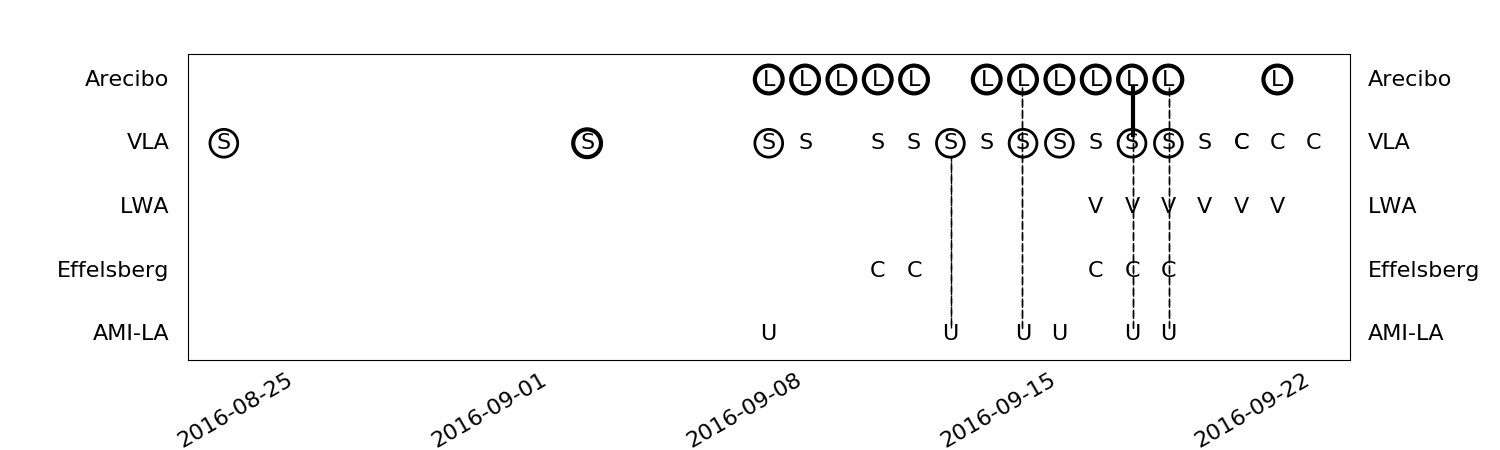
\includegraphics[width=2\columnwidth]{timeline}
\caption{Summary of observing coverage and detections of \frb\ during the multi-telescope observing campaign in August and September 2016. Symbols show days with observations and circles highlight observations that detected bursts from \frb. Multiple circles indicate multiple burst detections, except for Arecibo, which typically has multiple detections per observing session (a detailed analysis is left for a future paper). The black dashed lines show the VLA burst detections with simultaneous coverage at other telescopes. The solid black line shows the simultaneous burst detection at VLA and Arecibo.
\label{fig:multi}}
\end{center}
\end{figure*}

The data presented here were obtained from multiple programs and telescopes, but the central goal was to interferometrically localize \frb\ with the VLA. The observing strategy was to ensure simultaneous observing between the VLA and Arecibo observatories and add other observatories added on a best-effort basis. We coordinated observing between the VLA, Arecibo, Effelsberg, and AMI-LA telescopes, as shown in figure \ref{fig:multi}. Below, we summarize these observations, with a focus on those conducted simultaneously with VLA burst detections from \frb.

\subsection{VLA}
The \frb\ observing campaign started in late 2015 with a 10~hr campaign observed at 1.4~GHz in the compact D configuration. In April through May 2016, we conducted a 40~hr campaign at 3~GHz in the C and CnB configurations in coordination with Arecibo. We concluded with a new, 40~hr, coordinated campaign from August through September 2016 in the B configuration and during the move to the most extended A configuration. In this last campaign, the first 34 hours of VLA observations were made at 3~GHz, while the last 6 hours were observed at 6~GHz. This paper focuses on the data collected at 3~GHz, which includes all nine burst detections.

All VLA fast-sampled data were observed with 5~ms sampling, 256 channels, and dual-circular polarization \citep[as in]{2015ApJ...807...16L}. To maximize sensitivity, the channel frequency width was set to maintain sensitivity to the known DM of \frb, while maximizing the total bandwidth. The total bandwidth at L (1.4~GHz), S (3~GHz), and C (6~GHz) bands was 256~MHz, 1024~MHz, and 2048~MHz, respectively. The 3~GHz data were recorded data in 8 spectral windows with 32 channels each.

Observations in August and Septmeber were searched by a prototype version of \rf\footnote{See \url{http://realfast.io}.}. \rf\ is a real-time, fast imaging transient search system. The current, prototype runs on existing, CPU-based hardware of the VLA correlator backend, while the future \rf\ will run on a dedicated GPU cluster. The transient search pipeline software is called \emph{rtpipe}\footnote{See \url{https://github.com/caseyjlaw/rtpipe}} and is mostly written in Python (detail in \citet{2015ApJ...807...16L}). Images were formed for each integration at DMs of 0, 546, 556.9, 560, and 565 pc cm$^{-3}$. Gain calibration is read from the "telcal" system, which uses phase-only calibration on the previous gain calibrator. A flux scale is calculated for each spectral window from an observation on {\color{red} xx (Bryan)} and applied to all burst spectra.

Burst detections and localizations were made within hours of data being recorded. The transient search starts when data are recorded, but this prototype of \rf\ is a factor of several times slower than real-time, so we refer to the detection as "quasi real-time". Each image with a pixel higher than 6.4$\sigma$ is saved in a summary form as a check of data quality. For each image with a pixel higher than 7.4$\sigma$, \rf\ generates a more detailed candidate visualization with an image and spectrum. More detailed analysis, including improved calibration and localization, is conducted offline. 

Computational notebooks to reproduce the transient detection and localization can be found at \url{https://github.com/caseyjlaw/FRB121102}. Time cut-out visibility data are available at \url{https://doi.org/10.7910/DVN/TLDKXG}. Original visibility data are available under VLA program codes 16A-459 and 16A-496 and can be downloaded at \url{http://archive.nrao.edu}.

\subsection{Arecibo}

{\color{red} copied from the first paper}
During the joint Arecibo-VLA campaign, Arecibo observed with the L-wide receiver, which has an observational frequency range of 1.15 to 1.73~GHz and a full width at half maximum beam size of 3.3 arcmin. The PUPPI pulsar backend was used to record total intensity spectra with time and frequency resolutions of 10.24~$\mu$s and 1.5625~MHz, respectively, and full Stokes polarization information. Each frequency channel was coherently dedispersed to 557 pc cm$^{-3}$, thereby eliminating intra-channel dispersion smearing. PUPPI covers a total of 800~MHz of bandwidth centred at 1380.78125~MHz, but only $\sim$ 620~MHz of this band is usable due to radio frequency interference and receiver sensitivity roll-off at the band edges.

In total, twelve Arecibo observations had some simultaneous coverage with the VLA. Four of those observations were simultaneous with bursts detected with the VLA and one of those observations detected the same VLA burst. During the first VLA burst with Arecibo coverage (MJD 57643), the PUPPI system failed so data were recorded with {\color{red} xx (Jason?)} at C band. No detection was made in that Arecibo data. Overall, there were many more bursts detected at Arecibo than with the VLA and a more detailed analysis of those bursts will be presented in a future paper.

\subsection{Effelsberg}

{\color{red} copied from Laura's paper}
Observations were conducted at an observing frequency of 4.6 to 5.1~GHz. The S60mm receiver has a system equivalent flux density of 18 Jy and a full-width half-max (FWHM) beam size of 2.4\arcmin at 4.85~GHz. Pulsar search mode data were recorded with the PFFTS backend. Total intensity spectra were recorded with a time resolution of 65.5~$\mu$s and a bandwidth of 500~MHz divided into 128 frequency channels. Note, the inter-channel DM smearing time for 560~pc cm$^{-3}$\ is $\sim$0.2 msec at 4.6 GHz.

Five Effelsberg observations had some simultaneous coverage with the VLA, of which two were simultaneous with VLA bursts. Unfortunately, due to a configuration error, a 100~MHz bandwidth filter centered at 4.85~GHz was in place for both of these sessions. The sensitivity was about two times worse than the nominal value. No burst was detected in either observation.

\subsection{AMI}

We observed \frb with the Arcminute MicroKelvin Imager Large Array (AMI-LA; Zwart et al. 2008) for 3 hours each on four epochs starting at MJDs 57643.3351, 57645.3317, 57648.3352, and 57649.3353. Observations were made with the new digital correlator having 4096 channels across a 5 GHz bandwidth between 13--18 GHz with a 1s dump time. The phase calibrator, J0518+3306, was observed every 12 minutes for about 1.5 minutes. The AMI-LA data were binned to eight 0.625 GHz channels and processed (RFI excision and calibration) with a fully-automated pipeline, AMI-REDUCE \citep[e.g.,][]{2013MNRAS.429.3330P}. Daily measurements of 3C48 and 3C286 were used for the absolute flux calibration, which is good to about 10\%. 

We inspected the calibrated visibilities, and did not find any signal above 20 mJy in the 1s samples at and in the vicinity of the detected bursts. Concatenating and imaging the 12 hours of calibrated data with the CASA tasks {\it concat} and {\it clean} also does not yield any significant detection at the FRB location. Although the statistical 3sigma upper limit is 60 uJy, extended mJy-level sources in the field cause sidelobe confusion (the AMI-LA angular resolution is $\sim$30 arcsec), and the actual upper limit is larger. We introduced artificial point sources at the FRB location using the CASA {\it sm} tool, and found that these sources can be recovered as long as their peak flux densities are more than $\sim$100 uJy. Hence, we place an upper limit of 100$\pm$10 uJy on any quiescent or possible radio "afterglow" (on $\sim$days timescale) signal from the FRB. This limit is close to the flux density measured by the VLA \citep{LOC}.

\section{Results}

\subsection{Multi-Telescope Burst Spectrum}
Four of the VLA bursts were observed simultaneously with Arecibo and AMI-LA (Figure \ref{fig:multi}). Of these, the burst on 57648 was detected by Arecibo at the same time (after correcting for the known DM of \frb). The Arecibo detection of this burst had a significance of {\color{red} xx$\sigma$ (Jason)}.

Figure {\color{red} **to do**} shows the dynamic spectrum formed from the phased VLA and Arecibo data... **Discuss dispersion correction, time alignment, chance of false association** 

This simultaneous detection of a burst from roughly 1 to 4~GHz shows that some bursts cover more than an octave of frequency. However, this is one of three VLA bursts with coverage by Arecibo, so the other nondetections imply that those bursts had a smaller spectral width. In fact, as described in \S \ref{sec:spec}, many of the VLA bursts appear to be fully contained in the band from 2.5 to 3.5~GHz, which implies a much smaller spectral coverage for typical bursts.

%\begin{figure}[htb]
%\begin{center}
%\includegraphics[width=0.9\columnwidth]{}
%\caption{
%\label{fig:}}
%\end{center}
%\end{figure}

\subsection{VLA Bursts}

\begin{figure*}[htb]
\begin{center}
 \begin{minipage}{2\columnwidth}
  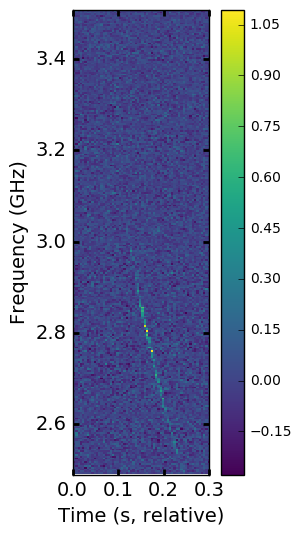
\includegraphics[width=0.18\columnwidth]{sgram_57623.png}
  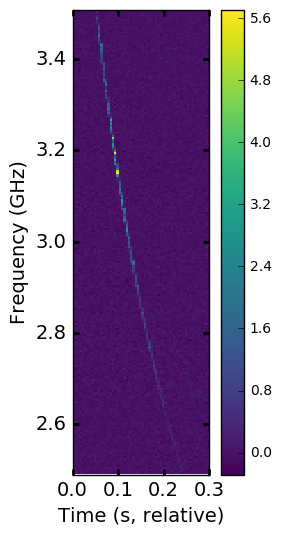
\includegraphics[width=0.18\columnwidth]{sgram_57633_scan7.png}
  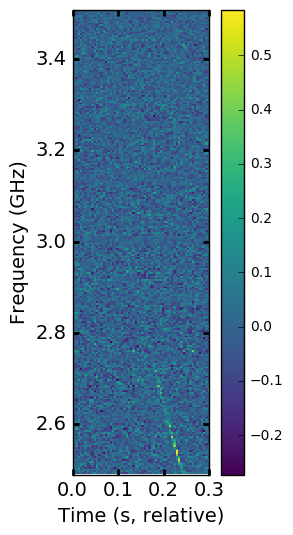
\includegraphics[width=0.18\columnwidth]{sgram_57633_scan13.png}
  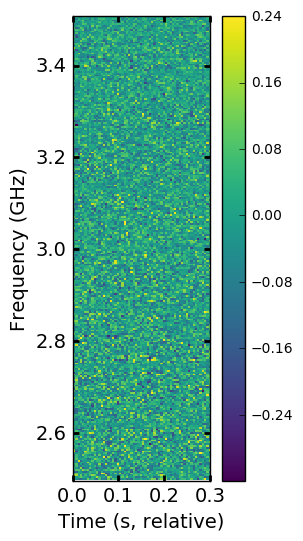
\includegraphics[width=0.18\columnwidth]{sgram_57638.png}
  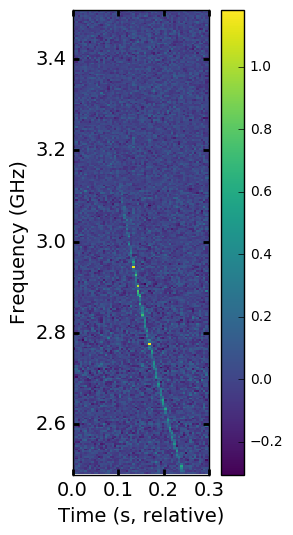
\includegraphics[width=0.18\columnwidth]{sgram_57643.png}
 \end{minipage}

 \begin{minipage}{2\columnwidth}
  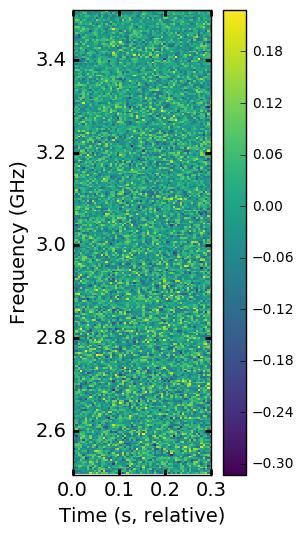
\includegraphics[width=0.18\columnwidth]{sgram_57645.png}
  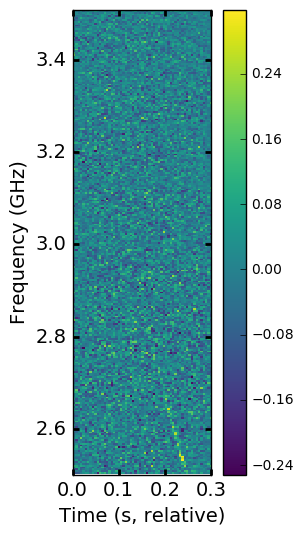
\includegraphics[width=0.18\columnwidth]{sgram_57646.png}
  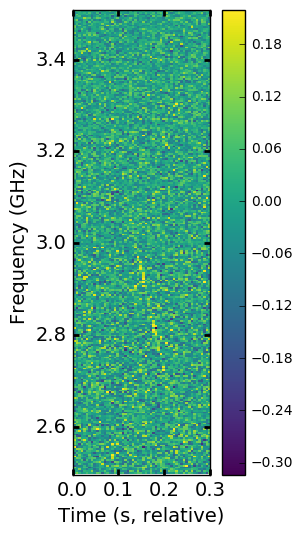
\includegraphics[width=0.18\columnwidth]{sgram_57648.png}
  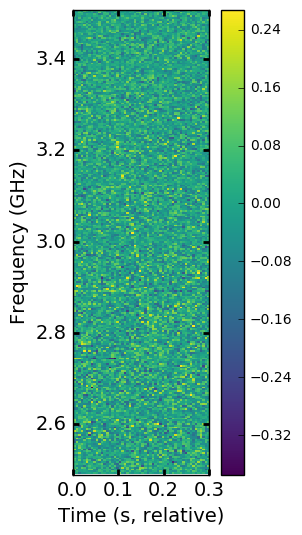
\includegraphics[width=0.18\columnwidth]{sgram_57649.png}
 \end{minipage}

 \caption{Dynamic spectra (time vs frequency intensity maps) for the nine VLA bursts. Starting at the top left, they correspond to bursts 57623, 57633.68, 57633.70, 57638, 57643, (bottom left) 57645, 57646, 57648, and 57649. Note that bursts are detected in 5~ms images generated from dedispersed visibilities.
 \label{fig:sgram}}
\end{center}
\end{figure*}


\subsubsection{Spectra}
\label{sec:spec}
Figure \ref{fig:sgram} shows the dynamic spectra of all nine bursts detected by the VLA. We improved on the initial analysis presented in \citet{LOC} by using a better calibration scheme and optimizing the detection significance over a fine grid of DM ($\Delta \rm{DM}=1 \rm{pc}\ \rm{cm}^{-3}$). Table \ref{tab:spec} shows the improved burst parameters using this new scheme. 

\begin{table*}
\caption{Properties of Bursts from \frb}
\centering
\begin{tabular}{lccccccc}
\hline
Date                & S$_{\rm{int}}$  & Image SNR & L$_{\rm{int}}$ & DM$_{\rm{opt}}$ & S$_{\rm{peak}}$  & Center & FWHM \\
(MJD)               & (mJy)           &           & ($10^{38}$\ erg) & (pc cm$^{-3})$ & (Jy) & (GHz)  & (MHz) \\ \hline
57623               & 258             & 38        & 15   & 561 & 0.41                                    & 2.8 & 300 \\
57633.68            & 2000            & 179       & 120  & 554 & 1.90                                    & 3.2 & 520 \\
57633.70\tablenotemark{a} & 105       & 15        & 6    & 559 & $>$0.188                                & $<$2.5 & $>$350 \\
57638               & 65              & 12        & 4    & 556 & 0.07                                    & 3.1 & 410 \\
57643               & 375             & 100       & 21   & 560 & 0.39                                    & 2.8 & 520 \\
57645               & 38              & 13        & 2    & 572 & 0.06                                    & 2.8 & 210 \\
57646\tablenotemark{a} & 69           & 20        & 4    & 555 & $>$0.16                                 & $<$2.5 & $>$400 \\
57648\tablenotemark{b} & 97           & 25        & 6    & 559 & 0.11                                    & 2.9 & 420 \\
57649               & 110             & 36        & 6    & 552 & 0.07                                    & 2.9 & 880 \\ \hline
\end{tabular}
\tablenotetext{a}{Best-fit Gaussian is not centered in 3~GHz band, so spectral parameters are limits.}
\tablenotetext{b}{Detected simultaneously with Arecibo between 1.15 and 1.73~GHz.}
\label{tab:spec}
\end{table*} 

Figure \ref{fig:spec} shows the spectrum of the integration and DM that maximizes the burst detection significance. After DM optimization, all bursts appear unresolved at the 5~ms time resolution of the VLA data. One possible exception is the brightest burst at 57633.68, for which roughly 10\% of the peak flux density is seen in adjacent 5~ms integrations.

\begin{figure*}[ht]
\begin{center}
 \begin{minipage}{2\columnwidth}
  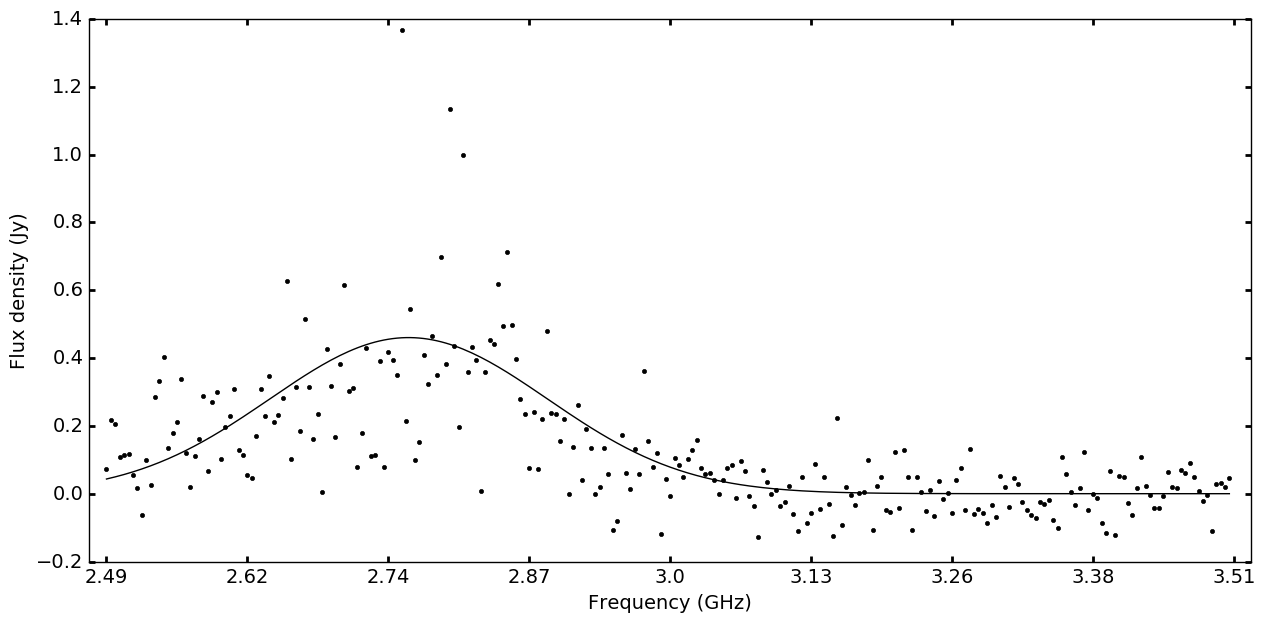
\includegraphics[width=0.3\columnwidth]{spec_57623.png}
  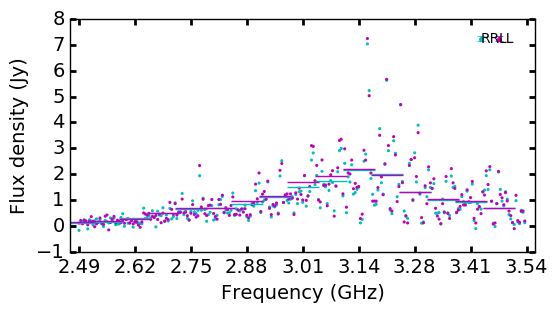
\includegraphics[width=0.3\columnwidth]{spec_57633_scan7.png}
  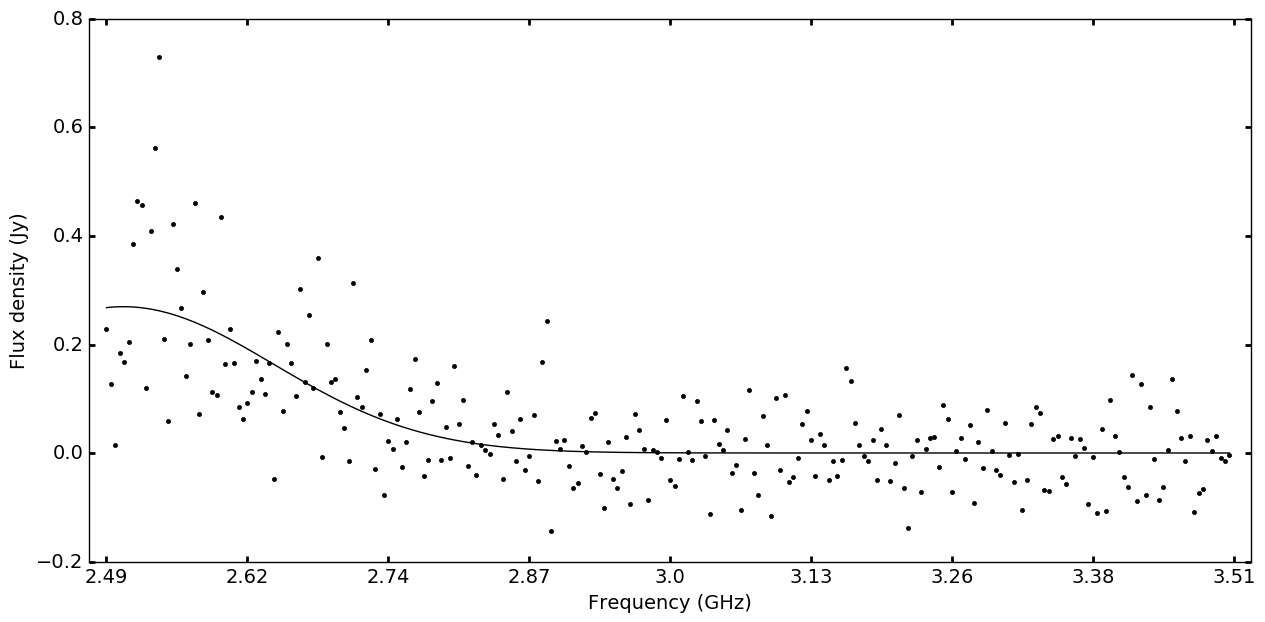
\includegraphics[width=0.3\columnwidth]{spec_57633_scan13.png}
 \end{minipage}

 \begin{minipage}{2\columnwidth}
  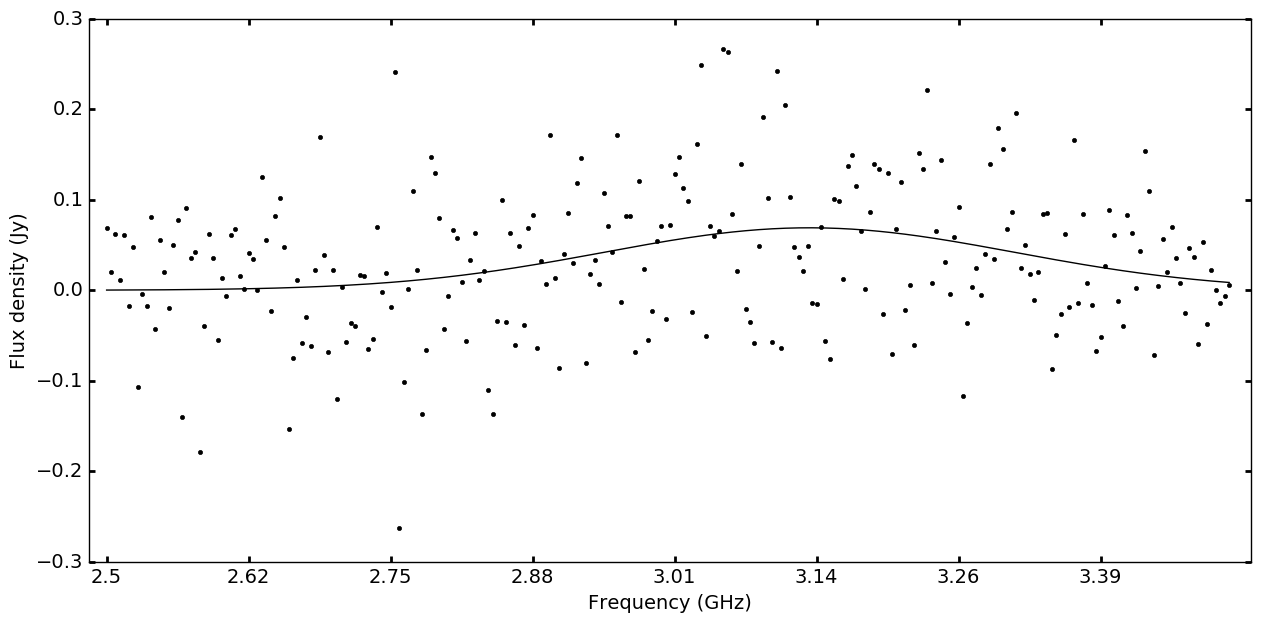
\includegraphics[width=0.3\columnwidth]{spec_57638.png}
  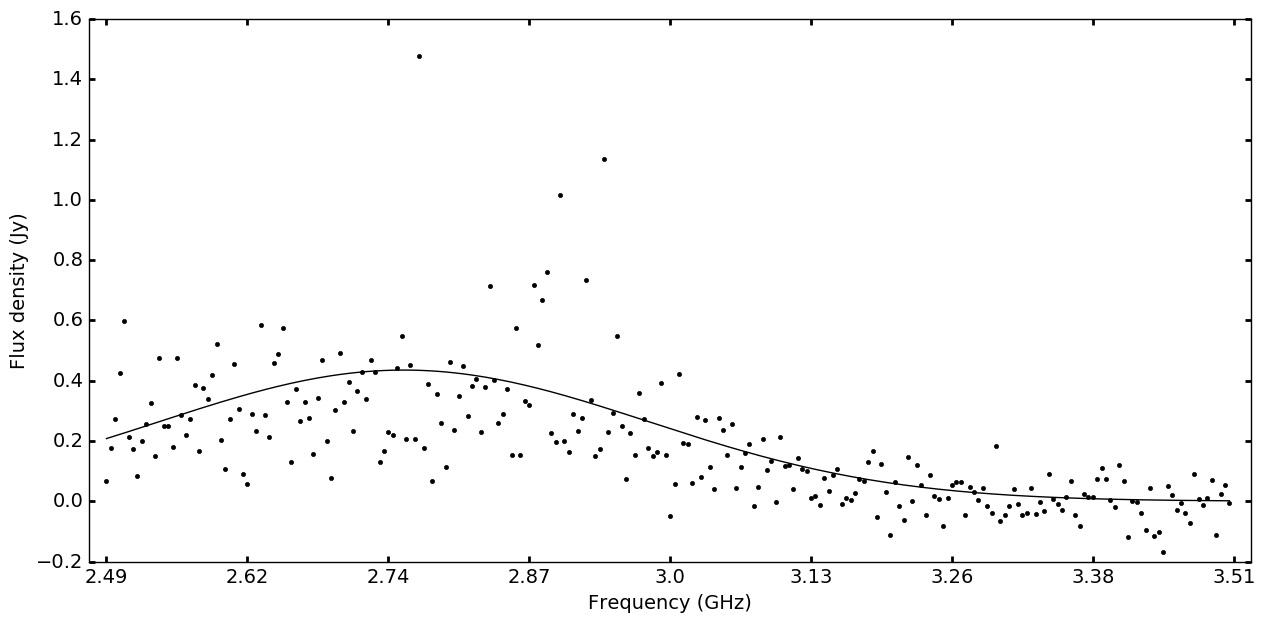
\includegraphics[width=0.3\columnwidth]{spec_57643.png}
  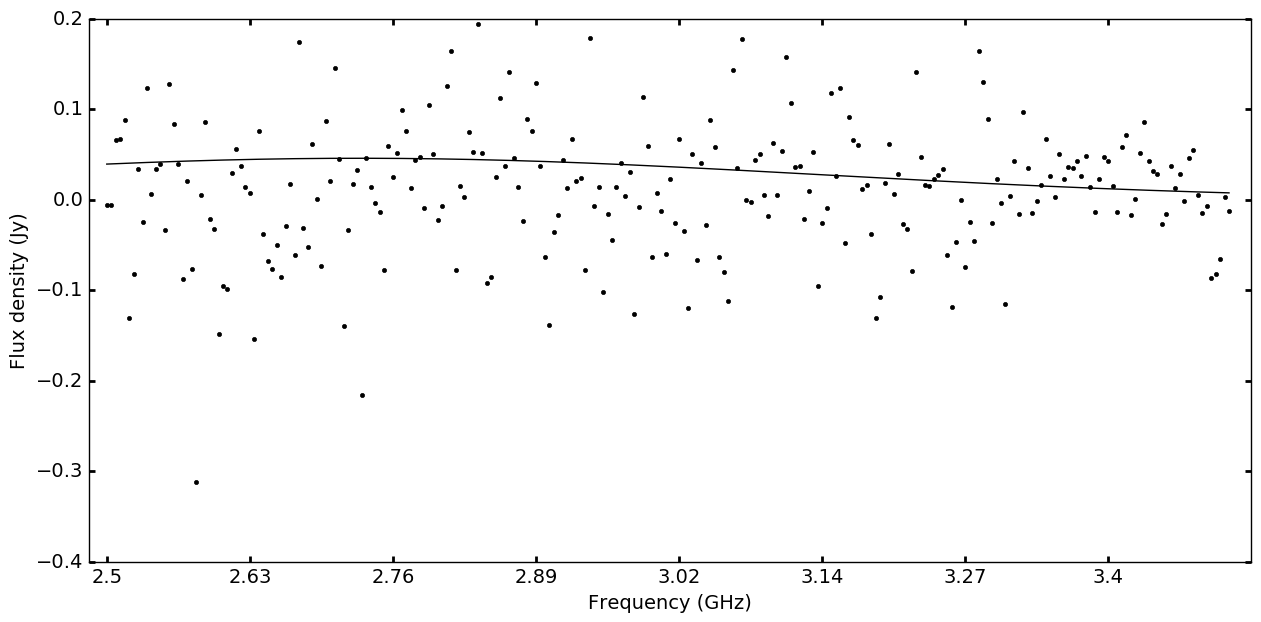
\includegraphics[width=0.3\columnwidth]{spec_57645.png}
 \end{minipage}

 \begin{minipage}{2\columnwidth}
  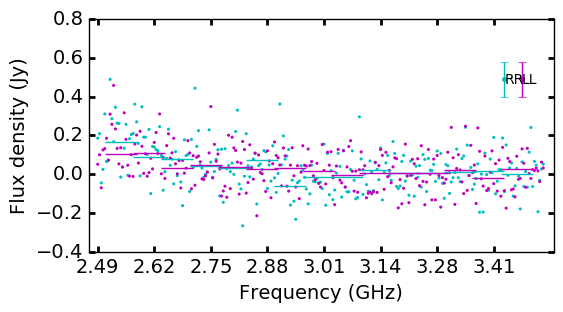
\includegraphics[width=0.3\columnwidth]{spec_57646.png}
  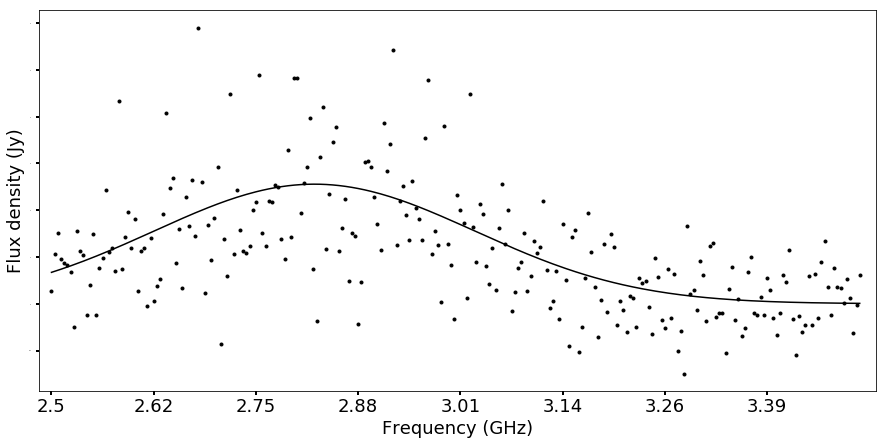
\includegraphics[width=0.3\columnwidth]{spec_57648.png}
  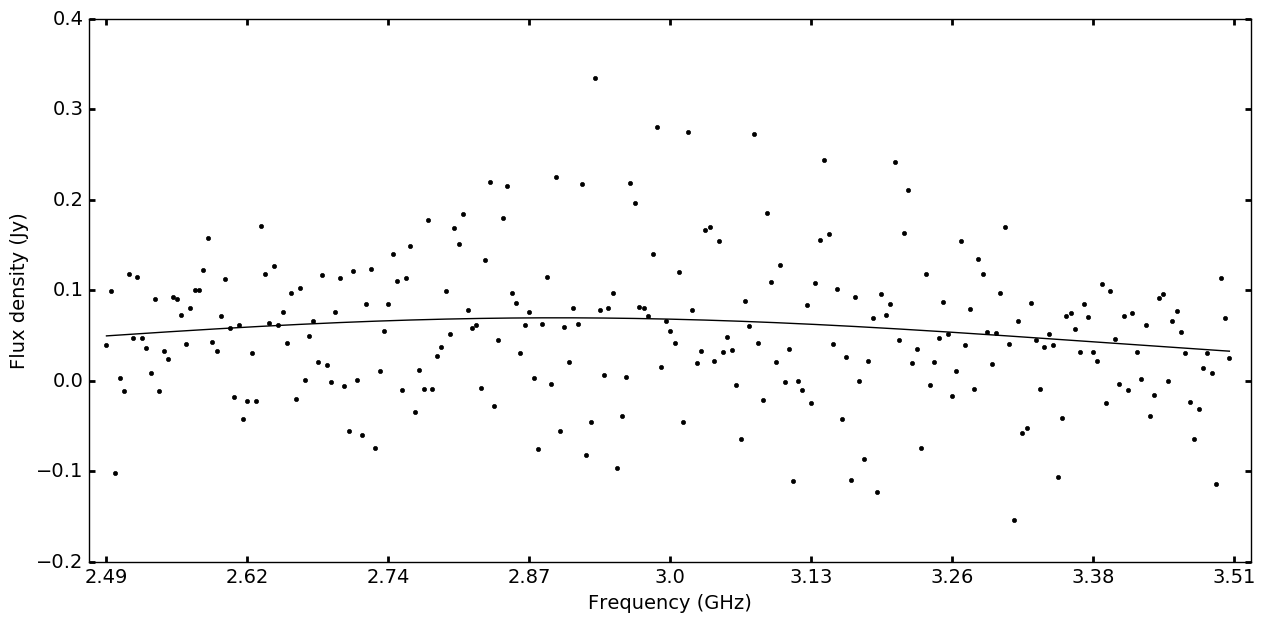
\includegraphics[width=0.3\columnwidth]{spec_57649.png}
 \end{minipage}
\caption{Spectra of nine bursts seen by the VLA from 2.5 to 3.5~GHz. Orthongonal circular polarizations (RR and LL) are plotted separately and example errorbars are shown at the top right of each panel. A binned spectrum is overplotted with a solid line.
\label{fig:spec}}
\end{center}
\end{figure*}

The burst spectra are generally characterized by a broad, Gaussian shape that with strong inter-channel modulation. We fit a Gaussian shape to each burst to estimate their characteristic width and peak flux, as summarized in Table \ref{tab:spec}. The channel-scale modulation is as high as 100\% (see \S \ref{sec:auto}) and is consistent with an exponential distribution. This introduces a strong bias to the best-fit Gaussian, but these simple fits are reliable enough to show that the typical burst has a spectral width of 500~MHz.
% TODO: fit with generative model with 100% amplitude modulations (emcee?)

All but two of the best-fit Gaussians are centered inside the 3~GHz band and most appear contained by the 1~GHz wide band. This is consistent with previous detections of \frb by Arecibo, which showed quasi-broadband structure \citep{2016arXiv160308880S} and large variation in the implied spectral index \citep{2014ApJ...790..101S}. A detailed discussion of high-resolution \frb\ burst spectra seen by the Arecibo Observatory will be presented elsewhere \citep{WEIRD}.

\subsubsection{Dispersion}
The initial VLA detections were made by searching a DM grid that allowed inter-DM sensitivity losses up to roughly 10\% \citep[$\Delta DM=10 \rm{pc}\ \rm{cm}^{-3}$][]{2003ApJ...596.1142C}. In optimizing detection significance over a fine DM grid, we find optimal DM values range from 552 to 572 pc cm$^{-3}$. However, the uncertainty in the peak DM measurement is defined by the DM sensitivity loss curve and the significance of the burst. 

Given that the apparent DM can potentially change due to intrinsic or extrinsic effects, we developed a more sophisticated system for modeling dispersion. We created a generative model to sample the likelihood distribution of a class of dispersion models \citep{2010arXiv1008.4686H}. We use the Gaussian shape (see \S \ref{sec:spec}) along the spectral axis and apply a frequency-depndent delay for a given dispersion model. The likelihood is directly sampled by calculating the product of probabilities on a per-pixel basis of the 2-dimensional dynamic spectrum. Uncertainties in each pixel are drawn from a uniform Gaussian error distribution that is estimated from the data.

 **Preliminary** Figure \ref{fig:dmmodel} compares the 95\% confidence intervals on the DM for all nine VLA bursts. The DM confidence intervals {\color{red} are/are not} consistent with a single DM... %, which suggests that there are apparent DM changes between bursts. This change could be caused by intrinsic burst structure or actual changes to the DM column density. 

High-resolution dynamic spectra at 1.4~GHz have discovered spectro-temporal structure that can bias the apparent DM differently from burst to burst \citep{WEIRD}. Observations at 1.4~GHz have measured DM in the range from xx to yy pc cm$^{-3}$, which is **smaller than/consistent with** the range of observed values seen by the VLA at 3~GHz. The FRB emission process has not yet been defined, so it is not clear how the intrinsic structure can bias DM as a function of frequency. {\color{red} Laura, any input from DM at higher frequencies?}

\begin{figure}[htb]
\begin{center}
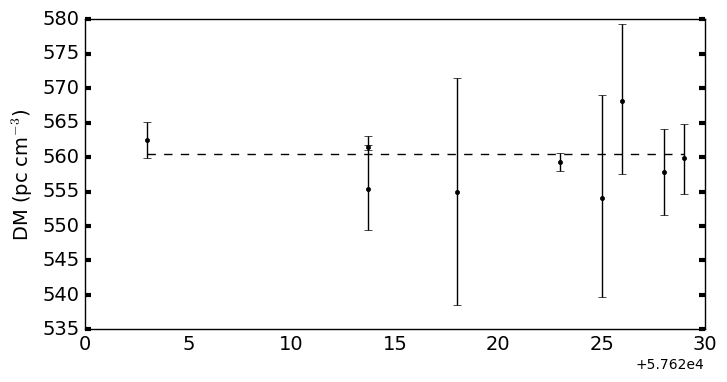
\includegraphics[width=0.9\columnwidth]{dmmodel}
\caption{**Preliminary** Comparison of 95\% ($1\sigma$) confidence intervals for DM for nine bursts detected by the VLA.
\label{fig:dmmodel}}
\end{center}
\end{figure}

% TODO: Non-lambda$^{2}$ dispersion...


\subsubsection{Spectral Autocorrelation}
\label{sec:auto}
Autocorrelation of the burst signal (both temporal and spectral) can be used to infer both intrinsic properties and modulation due to scintillation \citep{CORDES}. While VLA spectral resolution of 4~MHz is relatively coarse, the Galactic electron density model predicts a diffractive scintillation bandwidth of {\color{red} xx MHz at 3~GHz (Jim?)} \citep{2002astro.ph..7156C}. Figure \ref{fig:acf} shows the spectral autocorrellation for the strongest burst (MJD 57633.68). No excess correlation is found near the channel resolution, which limits the correlation width to less than 4~MHz.

\begin{figure}[htb]
\begin{center}
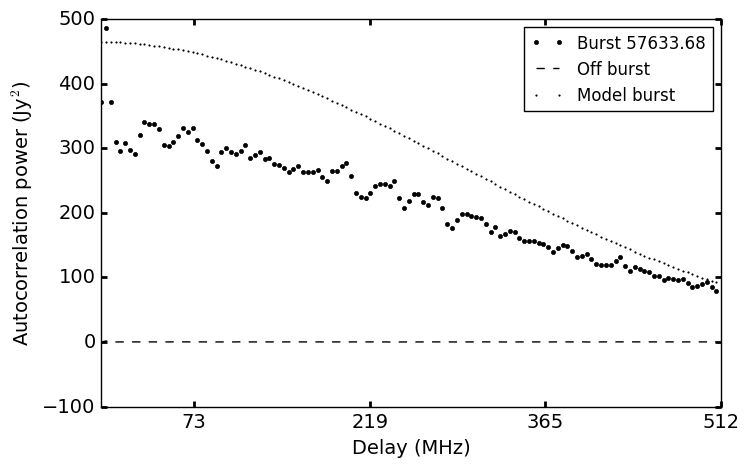
\includegraphics[width=0.9\columnwidth]{acf_57633_scan7}
\caption{The spectral autocorrelation for the burst from \frb\ at MJD 57633.68. Blue shows the autocorrelation for the burst and green shows an autocorrelation of a representative spectrum with no burst.
\label{fig:acf}}
\end{center}
\end{figure}

\subsubsection{Circular Polarization}
The VLA S-band recievers natively measure circular polarization, although for observing efficiency we chose not include polarization calibration procedures. Crude constraints on circular polarization are possible by comparing the burst intensity in right and left-hand polarized data products. The apparent circular polarization fraction ($(RR-LL)/(RR+LL)$) for the most significant bursts are all less than 3\%. \frb was located 2.3 arcmin away from pointing center, where systematic effects have been measured as large as 3\% (Perley et al 2016, VLA memo). Given that systematic effects dominate the apparent circular polarization, we conclude that the true fractional circular polarization is less than 3\%.

\subsection{Temporal Statistics}
\label{sec:temp}
Burst detections were made very inhomogenously through the larger (63 hours) observing campaign of FRB 121102. In the first 30 hours of observing at S-band no bursts were detected, while nine bursts were detected in the last 27 hours of S-band observing. The data quality is high, so the inhomogeneous burst distribution shows that the burst detection probability was not stationary. Assuming that the burst detection probability follows a Poisson distribution, the nondetection in the first half of S-band limits the FRB rate to $\rm{R}<0.1$ hour$^{-1}$ (95\% confidence limit). The mean detection rate for the last part of the campaign was $\rm{R}=0.3$ hour$^{-1}$.

There is weak evidence that the \frb\ burst rate changed during the last 27 hours of the S-band campaign. We modeled the event detection probability as a Poisson probability function, $P_i(\lambda)$, with rate parameter that evolves linearly in time relative to the first VLA burst $\lambda = a + b (\rm{MJD}_i - 57623)$. By directly sampling the joint probability distribution, $\prod_{i} P_i$, we can exclude a constant rate with $\sim$85\% confidence. This weak constraint is consistent with the broader trend seen by the VLA and Arecibo.

%\begin{figure}[htb]
%\begin{center}
%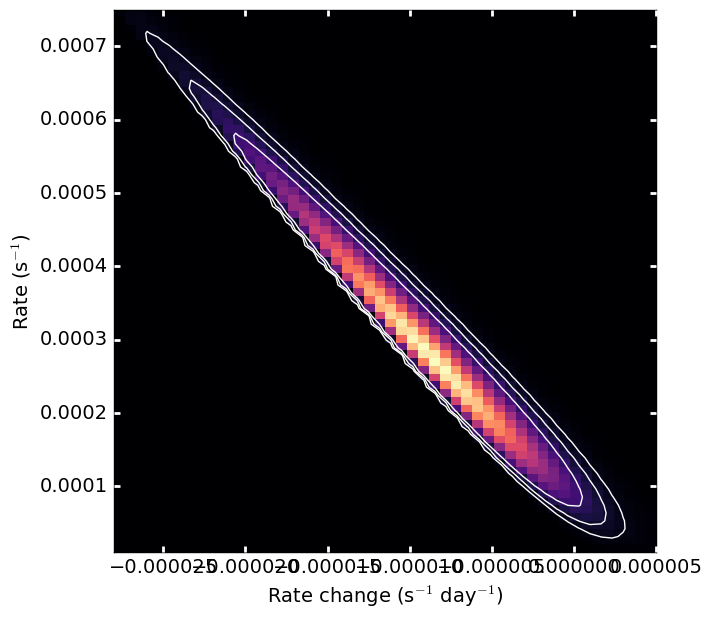
\includegraphics[width=0.9\columnwidth]{event_rate_contours}
%\caption{Color scale and contours show the relative probability for a time-evolving Poisson detection probability for \frb. Contours show the 50, 90, and 95\% confidence contours on the rate $a$\ (bursts s$^{-1}$) and rate change $b$\ (bursts s$^{-1}$ day$^{-1}$) during the August--September 2016 campaign in which bursts were detected.
%\label{fig:rate}}
%\end{center}
%\end{figure}

During the August--September 2016 observing campaign, the typical observation lasted about two hours and was sampled with a 5~ms cadence. We used the Lomb-Scargle periodogram \citep{1982ApJ...263..835S} to search for periodic structure over a wide range of timescales. The time series is calculated by binning the burst detection rate per 100~ms \citep[always either 0 or 1, see also]{2011MNRAS.417.1871P}. 
The spectral power calculated for periods between 0.8 and 80 s shows no power in excess of the typical 95\% confidence bound estimated from shuffled data. We verified that simulating nine bursts drawn from a simple rotational model would produce excess power using this approach. However, it is difficult to put strong constraints on more complex rotational models \citep[e.g., with wide pulse phase windows or glitches][]{2007ApJ...663..497C, 2013Natur.497..591A}

\subsection{Luminosity and Brightness Distribution}
\label{sec:disn}
Knowing the burst distance, we calculate their mean luminosity across a single 5~ms integration and the 1~GHz bandwidth (Table \ref{tab:spec}). The VLA has also shown for the first time that most bursts are contained within the 3~GHz band. That means that the mean S-band flux density can be converted to a luminosity in units of ergs with no assumptions about its spectral properties.

This uniform sample of burst luminosities can be used to infer more general properties of \frb. We treat the detection probability as a Poisson process with a rate that scales with the luminosity as a powerlaw. Figure \ref{fig:lumd} shows the probability distribution for the powerlaw amplitude and index for the sample of nine VLA bursts. The luminosity powerlaw index $1\sigma$ bounds range from --0.5 to +0.4; for a cumulative luminosity distribution, this corresponds to a powerlaw index of roughly --0.6. The flatness of the distribution is also clear from range of significance of the nine bursts (12 to 179$\sigma$). All bursts are much brighter than the sensitivity limit, so the distribution is not affected by a completeness limit.

\begin{figure}[htb]
\begin{center}
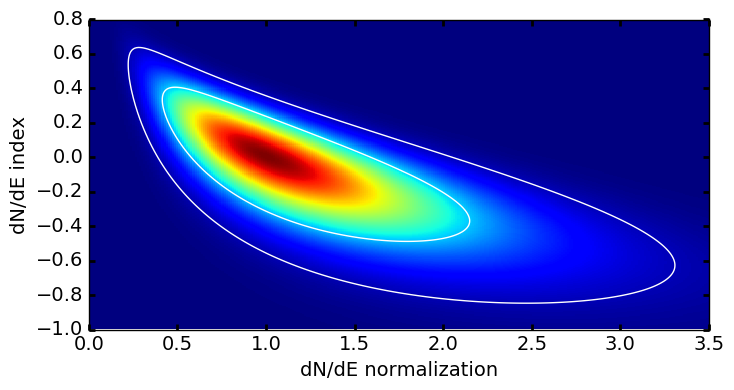
\includegraphics[width=0.9\columnwidth]{luminosity_disn}
\caption{Probability distribution of powerlaw luminosity model for the nine VLA bursts from \frb. Powerlaw referenced to $L=2\times10^{38}$\ erg.
\label{fig:lumd}}
\end{center}
\end{figure}

Assuming that \frb\ is representative of the overall FRB population, we can use the luminosity distribution of the former to infer properties of the latter. The primary observable of the FRB population is the flux distribution. We use a Monte-Carlo technique to simulate an FRB population with a given luminosity and spatial distribution. To reproduce the observed FRB sample, we select the brightest $N$\ bursts and fit their fluxes with a powerlaw. The tail of this distribution selects for extrema, such cut-offs in the intrinsic distribution or propagation effects \citep{2015MNRAS.451.3278M, CORDES}. Therefore, we sample 100 such populations and measure 95\% bounds on the distribution of cumulative flux distribution index.

These simulations confirm previous work that shows that in many circumstances the cumulative flux distribution follows a Euclidean distribution \citep[index = --1.5;][]{2016MNRAS.462..941L}. To reproduce the flatness (index$\approx-1$) of the observed flux distribution, we need to incorporate other effects. 
**in progress** (new figure?)


\section{discussion}

\subsection{Emission Physics and Burst Energetics}
The measurement of a redshift to the host of \frb allows us to measure the burst luminosity. We now know that \frb\ is detectable with the VLA out to $z=0.7$ and much farther with Arecibo. This confirms the results presented in \citet{LOC}, which quoted a luminosity on the order of $10^{38}$\ erg. The more refined analysis presented here measures somewhat higher burst fluxes, so the brightest VLA burst luminosity is now on the order of $10^{40}$\ erg. 

However, the total energy emitted by \frb\ can be orders of magnitude different than this isotropic, apparent luminosity. While the emission process is not yet known, it is neccessarily coherent \citep{2016Natur.531..202S, WEIRD}, so relativistical beaming will amplify the apparent brightness. Propagation effects (e.g., scintillation, scattering) can also modify the radio signal in a variety of ways \citep{CORDES} and the duration of the emission in the source frame is not known. In any case, the luminosity scale is still larger than any Galactic class of fast radio transient and requires either a new process or dramatic scaling of known emission processes \citep{2016MNRAS.462..941L, 2016MNRAS.457..232C}.

\subsection{FRB Flux Distribution}
Doubts were cast on the first FRB detection (``Lorimer burst'') due to its unusually high brightness. The lack of lower-significance detections suggested that this burst was unlikely to be part of any astrophysical population. With more detections, it has become clear that the FRB population has a relatively flat flux distribution \citep{2016ApJ...830...75V, 2016arXiv160206099L, 2016arXiv161100458L}. This fact was recently demonstrated by yet another detection of an extremely bright FRB \citep{2016arXiv161105758R}.

**Discussion of luminosity/flux distribution analysis presented in \S \ref{sec:disn})**

It is not yet clear whether \frb\ can be treated as a representative of the broader FRB population. \citet{2016Natur.531..202S} describes burst spectral structure that is intrinsic, or at least dominated by propagation effects close to the emitting region. On the other hand, \citep{CORDES} have identified a variety of propagation effects in our own Galaxy that can plausibly modify the observed brightness distribution.

\subsection{Repetition}
The burst rate analysis presented in \S \ref{sec:temp} shows that the detection probability of \frb\ is not stationary. As mentioned above, this could be caused by intrinsic events (e.g., magnetar outburst) or propagation effects. In either case, it demonstrates that \frb\ has a kind of "red spectrum" temporally, in which bursts tend to cluster in time \citep{2016MNRAS.458L..89C}. The detection of a burst improves odds of finding more bursts in near-future observations. 

If this statistical property describes other FRBs, it weakens previous constraints on repetition \citep{2015MNRAS.454..457P,2015ApJ...807...16L}. It is possible that other FRBs have repeating bursts, although calculating a limit requires knowing the temporal powerlaw that defines the repetition. Observations of \frb\ have not yet detected enough bursts to reliably measure that index. This repetition also implies that there are fewer phyiscal sources of FRBs than implied by the burst detection rate.

\subsection{FRB Rate}
% cut from gemini paper. TODO: incorporate referee comments on rate scale. Sarah?
Assuming that \frb is from the same population as the other FRBs, the measurement of a distance for the host of \frb allows us to re-evaluate the cosmic volume and event rate per galaxy for the FRB population. The estimated projected FRB rate $R_p$ understates the true rate by a beaming fraction $\Omega_b$ \citep[$\sim$10\%;][]{1998MNRAS.298..625T}.. For a comoving volume $V(z)$ and galaxy number density $\Phi(M)$, the rate per galaxy is $R_{FRB} = R_p /(\Omega_b \Phi(M)V (z))$. 

The first such rate estimate was made by \citet{2013Sci...341...53T}, who used the measured DM to estimate a characteristic distance for their sample of 4 FRBs. They assumed that all of the extragalactic component of the DM was caused by the IGM and scaled as $DM\approx z\times1200 \rm{pc}\ \rm{cm}^{-3}$ \citep{2003ApJ...598L..79I,2004MNRAS.348..999I}. They also calculated the number of galaxies by assuming a characteristic $L_*$ galaxy \citep[corresponding to stellar mass $M_* \approx 1010.66 M$][]{2012MNRAS.421..621B}.

Our calculation differs in that we have better estimates of all three parameters. First, the projected FRB rate is now believed to be closer to $2\times10^3 \rm{sky}^{-1} \rm{day}^{-1}$\ at high Galactic latitudes and flux densities brighter than 1 Jy ms \citep{2016arXiv161100458L,2016MNRAS.460L..30C}. \frb\ is associated with a relatively small galaxy, which are roughly a factor of 100 more abundant \citep[$\Phi(M) \approx 10^{-2} \rm{Mpc}^{-3}$;][]{2007ApJ...665..265F}. Finally, the measured distance for FRB 121102 suggests that roughly half of the extragalactic DM is intrinsic to the host and half is from the IGM.

This reduces the characteristic distance by a factor of two and the volume by an order of magnitude. Considering these factors, we assume a characteristic FRB redshift of 0.4 to estimate $R_{FRB} \approx 10^{-4} (0.1/\Omega_b) \rm{galaxy}^{-1} \rm{year}^{-1}$, which is two orders of magnitude lower than previously estimated \citep[assuming isotropic radiation;]{2013Sci...341...53T}.

There are significant caveats to the comparison of this rate to the rates of other classes of transient. This isotropic FRB rate assumes a projected FRB rate at a single (observationally defined) flux limit and that no bursts repeat. Using this calculation with data from more sensitive telescopes, we might infer a higher rate. However, if we assume that \frb\ is representative of the overall FRB population, then more sensitive observations would be more likely to find repeating FRBs that would effectively depress the estimate of the underlying isotropic rate per source. In this model, these two effects partially cancel, although without a physical model it is difficult to say how well.

\subsection{Observing Strategies}
As discussed above, \citet{2016MNRAS.458L..89C} note that the FRB repetition implies that the number of FRB-generating sources is smaller than the number of bursts. In some scenarios, this means that there are areas on the sky that may contain no FRBs. Wide, shallow surveys are the preferred strategy for blind detection of FRBs. However, future efforts to localize FRBs are still most likely to success by targeting known FRBs to catch repetitions. Finally, we note that the spectral coverage of bursts from \frb\ are relatively narrow ($<1$~GHz) and change dramatically between bursts. Thus, the odds of detecting a burst will improve linearly with bandwidth for bandwidths wider than this characteristic scale.

\subsection{Naming Convention}
The consistency of \frb\ properties (e.g., luminosity distribution) with the overall population suggests other FRBs likely repeat. If so, the current naming convention for FRBs (analogous to cataclysmic supernovae), will likely become uninformative, especially as large FRB survey projects come online \citep{2014SPIE.9145E..22B}. If all FRBs repeat, then a more useful convention would be based on coordinates. However, there are already two FRBs that have consistent celestial positions and different DMs. Therefore, we suggest an FRB naming convention as Jhhmm+ddDMmmmm.

\section{Conclusions}
Prior to being established as a cosmological source, the low Galactic latitude of \frb\ made it a somewhat compromised member of the FRB class. With its cosmological distance firmly established, \frb\ now serves as a new kind of standard by which FRBs are defined. 


 % include timeline and science scope for new localizations? realfast plug and reference cosmology papers, contingency on DMhost, etc.

\bibliographystyle{apj}

\section*{Acknowledgements}
We thank ...
This project was supported by the University of California Office of the President under Lab Fees Research Program Award 237863. The National Radio Astronomy Observatory is a facility of the National Science Foundation operated under cooperative agreement by Associated Universities, Inc.. This research made use of Astropy, a community-developed core Python package for Astronomy (Astropy Collaboration, 2013).

\bibliography{fasttrants.bib}

%\begin{figure}[htb]
%\begin{center}
%\includegraphics[width=0.9\columnwidth]{}
%\caption{
%\label{fig:name}}
%\end{center}
%\end{figure}

%\begin{table}
%\caption{Caption}
%\footnotesize
%\centering
%\begin{tabular}{l|cc|cc|c}
%\hline
%Field       & RA          & Dec   & Lon. & Lat.     & Time \\
%            & \multicolumn{2}{|c|}{(J2000)}  & \multicolumn{2}{|c|}{(Galactic; deg)} & (hrs) \\ \hline
%RA02        & 2:27:53  &  +9:13:24 & 159.0 & --46.8    & 26.25 \\
%PSR J2248-0101 & 22:48:27 & --1:1:48 & 69.3 & --50.6 & 6.5 \\ \hline
%\end{tabular}
%\label{fields}
%\end{table} 

\end{document}

